% 本章对应赛题问题四。事实依据：仓库 main@f3a49d4 的 Q4 实现、实验与输出。
% 图件由用户提供；所列未来月份均从附件中的最后提交日期起算。
\setcounter{section}{6}
\section{问题四：技术演进分析与前沿预测}
\label{sec:q4}
\setcounter{equation}{0}
\setcounter{figure}{0}
\setcounter{table}{0}

\subsection{问题分析与数据整理}

本问需要回答两个相互关联的问题：历史能力增长中，模型规模变化与同规模条件下的变化分别占多少；若算力增速放缓，未来一至两年开源模型的高端能力和最高能力可能达到什么水平。前三问以交叉熵 Loss 度量模型表现，而本问以多项 Benchmark 得分度量能力，因此还需建立来源一致的 Loss--能力关系\cite{gadre2024,observational2024}，分析前述配置在能力坐标上的含义。

令模型 $i$ 的综合能力为 C2 六项得分的等权均值
\begin{equation}
 S_i=\frac{1}{6}\sum_{k=1}^{6}s_{ik},\qquad 0\leq S_i\leq100,
 \label{eq:q4-score}
\end{equation}
六项分别为 IFEval、BBH、MATH Lvl 5、GPQA、MUSR 和 MMLU-PRO\cite{mmlupro2024}。仅当六项均有有效得分时计算 $S_i$。时间轴采用榜单提交日；模型类型分为基础预训练和后训练两组，后者包含 chat 与领域微调。开放模型筛选排除明确标注不开放权重的记录，并结合权重及许可证标签；严格开放和许可证口径另作敏感性比较。许可证标签只能作为开放可用性的筛选依据，具体研究与复现权限仍由对应许可证决定。对同名模型在当期分析中保留最新提交版本，但计算历次最高分时保留所有历史版本。

表\ref{tab:q4-data}概括本问的数据角色。C2 去重后的扩展开放集合为 2616 个模型，其中主分析使用基础预训练 204 个、后训练 1620 个。C3 的 4599 行记录来自不同评分来源和年份；其中历史报告的 26 行原有 Average 与式\eqref{eq:q4-score}所算六任务均值的平均绝对差为 9.101 分，因此按来源、年份和任务分别分析，不把不同口径的 Average 拼接成同一能力曲线。C8 的 1860 个可解析模型均有 24 项 BBH 任务结果。逐模型聚合后，BBH 宏平均的中位数为 49.40 分，而任务最低分的中位数为 14 分，1368 个模型至少有一项任务低于 20 分，说明综合均分会掩盖任务短板。C7 提供 2048、8192 和 131072 Token 三档已观察到的上下文长度，作为与第三问衔接的配置情景；最高一档仅有一个对应模型，不用于估计上下文长度的独立能力效应。

\begin{table}[htbp]
 \centering\small
 \caption{问题四的数据来源与分析用途}
 \label{tab:q4-data}
 \begin{tabular}{lp{4.0cm}p{6.4cm}}
 \toprule
 来源 & 数据性质 & 本问用途\\
 \midrule
 C2 & 六项能力得分、类型、提交日、开放标签 & 定义能力、历史分解、前沿回测及预测\\
 C3 & 多来源历史能力记录 & 分来源和逐任务考察长期变化，核对评分口径\\
 C4 & 参数量、训练量、算力与开放权重信息 & 估计资源增长情景并比较筛选口径\\
 C6 & Loss 与能力的成对记录 & 在各自来源内建立 Loss--能力关系\\
 C7 & 模型架构及上下文长度记录 & 确定跨问题配置所用的上下文情景\\
 C8 & BBH 原始逐任务结果 & 检查任务分布与均分掩盖的短板\\
 \bottomrule
 \end{tabular}
\end{table}

在 C3 的同一现代榜单来源内，2024 年和截至附件截点的 2025 年提交样本，六任务均分的第 90 百分位分别为 35.108 和 39.665 分；其中 MATH Lvl 5 的单任务第 90 百分位由 32.175 升至 45.846 分。按上述重复键去重后，两年六任务第 90 百分位为 35.100 和 39.626 分，变化很小。历史论文报告组则存在较高的任务零值比例与不同的 Average 口径，故它用于观察各项任务的历史覆盖和得分差异，不与现代榜单直接拼接预测。

C4 的 3523 条资源记录中，$N,C,D$ 均为正且有限的有 850 条。进一步按生成式语言任务、显式开放权重、Token 单位、基础模型、架构和来源可靠性筛选，并以 $C/(6\times10^{18}ND)\in[0.5,2]$ 检查资源单位的一致性，得到主集合 81 条；将最后一项放宽为 $[0.1,10]$，得到 93 条。这里 $N,D$ 分别以十亿参数和十亿 Token 计，$C$ 为 FLOPs。计算量有些本就由 $N,D$ 估算，因此上述比值用于核对口径。对 2021--2024 年各年算力的第 90 百分位取常用对数并拟合年度趋势，主集合的年增速为 $g_C=0.690315$ 个十进对数单位，即年倍率约 4.901；放宽集合分别为 0.600552 和 3.986。图\ref{fig:q4-resources}显示两种筛选下的资源变化。后续把这些速率作为未来投入情景，不直接解释为能力增长的因果系数。

\begin{figure}[htbp]
 \centering
 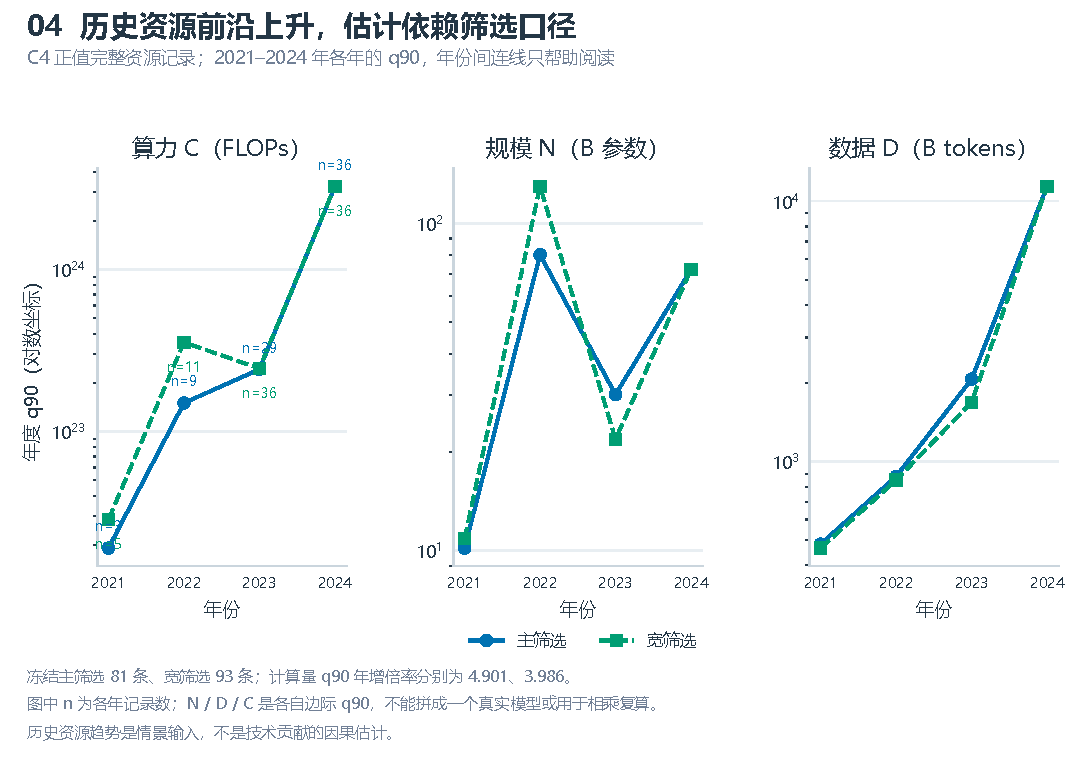
\includegraphics[width=0.84\linewidth]{figures/Q4/04_resources.pdf}
 \caption{两种筛选口径下的历史算力、参数量和训练量上沿}
 \label{fig:q4-resources}
\end{figure}

\subsection{历史能力变化的标准化分解}

\subsubsection{规模分布与同格变化}

为比较规模扩张和其余变化，在相同模型类型内分别取最早与最晚的两个月样本，按 $\log_{10}N$ 划分参数格，要求每格两期均至少有两个模型。后训练组中的 chat 与领域微调先分别处理，再使用两期合并样本形成固定类型权重 $\pi_g$。设 $w_{gjt}$ 为类型 $g$ 内参数格 $j$ 在时期 $t$ 的样本权重，$m_{gjt}$ 为该格能力均值，定义共同支持上的标准化均值 $M_t=\sum_g\pi_g\sum_jw_{gjt}m_{gjt}$。对 $M_1-M_0$ 作对称分解：
\begin{align}
 \Delta_{\rm scale}
 &=\frac12\sum_g\pi_g\sum_j(w_{gj1}-w_{gj0})(m_{gj1}+m_{gj0}),
 \label{eq:q4-scale-term}\\
 \Delta_{\rm within}
 &=\frac12\sum_g\pi_g\sum_j(w_{gj1}+w_{gj0})(m_{gj1}-m_{gj0}),
 \label{eq:q4-within-term}\\
 \Delta_{\rm std}&=M_1-M_0=\Delta_{\rm scale}+\Delta_{\rm within},\nonumber\\
 \Delta_{\rm gap}&=\Delta_{\rm full}-\Delta_{\rm std}.
 \label{eq:q4-gap}
\end{align}
第一项衡量样本在参数格间移动所造成的均分变化，第二项衡量相同格内的变化；全样本与共同支持结果之差单独留在 $\Delta_{\rm gap}$。这一恒等式避免将样本组成和支持范围变化误计入某一贡献。

表\ref{tab:q4-decomp}给出 $0.5$ decade 参数格的主结果。后训练组的共同支持均分由 18.937 升至 24.700，增量 5.763 分；参数分布项为 $-0.758$ 分，同格变化为 $6.521$ 分。相对标准化增量，两项带符号份额分别为 $-13.15\%$ 和 $113.15\%$。超过 100\% 的份额源于规模分布项的反向抵消。若假定同格内训练量、后训练投入和评测选择近似稳定，可将前者视为可见规模变化的贡献，后者视为非规模变化的剩余贡献。附件缺少与 C2 逐模型对齐的 $D$ 及训练过程信息，故同格项也可能包含数据量、后训练和样本选择的变化。基础组的标准化增量仅 0.880 分，其比例对小分母较敏感，表中保留分值而不汇总总体百分比。图\ref{fig:q4-contributions}直观展示三项如何组成全样本增量。

\begin{table}[htbp]
 \centering\small
 \caption{两月窗口、$0.5$ decade 参数格下的能力变化分解（分）}
 \label{tab:q4-decomp}
 \begin{tabular}{lrrrrrr}
 \toprule
 类型 & 共同支持早/晚 & 标准化变化 & 参数分布 & 同格变化 & 支持差 & 全样本变化\\
 \midrule
 后训练 & 313/423 & 5.763 & $-0.758$ & 6.521 & $-1.542$ & 4.222\\
 基础预训练 & 78/41 & 0.880 & $-3.756$ & 4.636 & $-2.072$ & $-1.192$\\
 \bottomrule
 \end{tabular}
\end{table}

\begin{figure}[htbp]
 \centering
 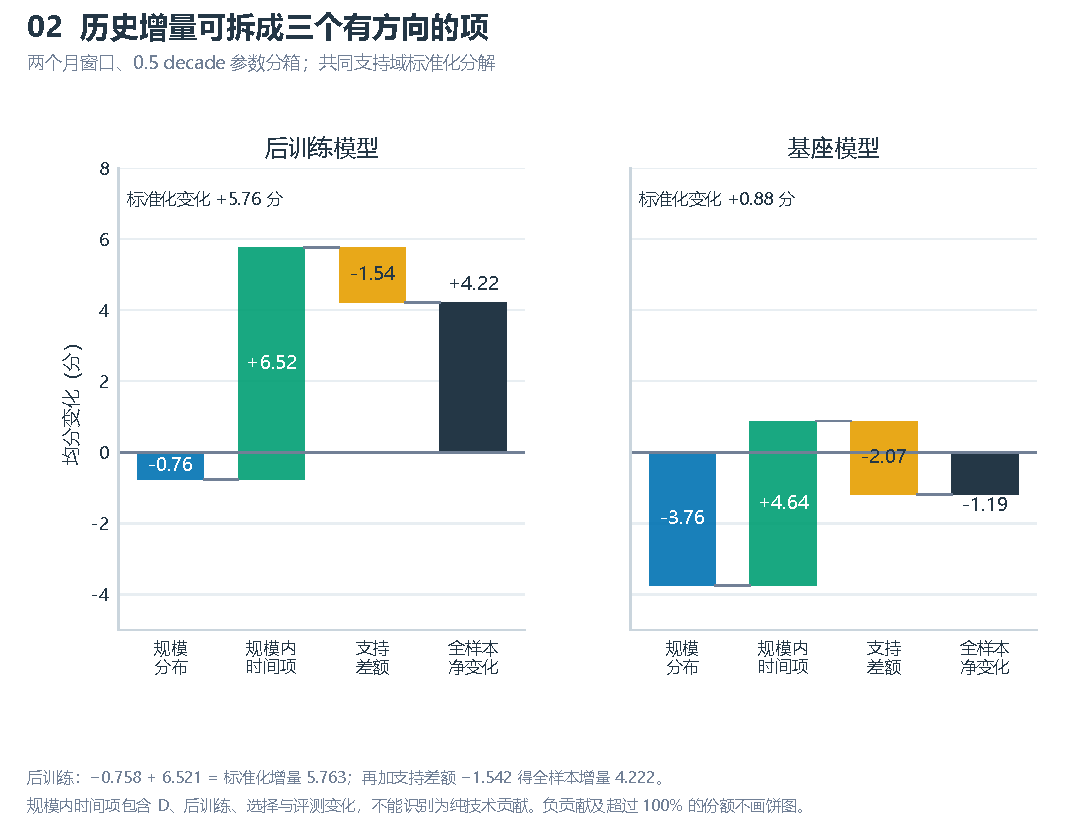
\includegraphics[width=0.84\linewidth]{figures/Q4/02_contributions.pdf}
 \caption{两类模型历史能力增量的参数分布、同格变化及支持差}
 \label{fig:q4-contributions}
\end{figure}

\subsubsection{分解结果的敏感性}

改变参数格宽与样本窗口可考察分解对共同支持划分的依赖。在两月窗口下，后训练组采用 $0.25$、$0.50$、$0.75$ decade 参数格时，规模分布份额依次为 $-16.47\%$、$-13.15\%$、$-50.08\%$：在主开放口径内符号相同，幅度变化明显，见图\ref{fig:q4-decomp-sensitivity}。再以开发者为抽样块重复抽取 80 次，主格宽下参数分布项的第 5 至第 95 百分位为 $-2.329$ 至 $0.257$ 分，跨过零；同格项对应为 $4.679$ 至 $8.460$ 分。若进一步只比较相同开发者的共同参数格，后训练组两期仅保留 6 和 8 个模型，难以据此估计总体中排除开发者差异后的变化。

开放模型的筛选口径也会改变贡献分解。表\ref{tab:q4-open-sensitivity}在相同的两月窗口和 $0.5$ decade 参数格下比较三种口径。主口径与明确标注开放权重的严格口径中，参数分布项均为负；仅按宽许可证标签筛选时，该项转为正值。这说明 $-13.15\%$ 是主样本条件下的参数规模份额，不能视为所有开放筛选方式下不变的比例；相较之下，三种口径的同格变化项均为正。结合抽样结果，历史得分提高的主要数值部分来自同参数格内的变化，但其中仍混有训练数据量、后训练方式和入榜选择的影响。

\begin{table}[htbp]
 \centering\small
 \caption{开放筛选口径对后训练组贡献分解的影响（两月窗口，$0.5$ decade）}
 \label{tab:q4-open-sensitivity}
 \begin{tabular}{lrrrrr}
 \toprule
 筛选口径 & 共同支持早/晚 & 标准化变化 & 参数分布 & 同格变化 & 参数份额\\
 \midrule
 主口径 & 313/423 & 5.763 & $-0.758$ & 6.521 & $-13.15\%$\\
 明确开放权重 & 31/58 & 6.758 & $-0.362$ & 7.121 & $-5.36\%$\\
 宽许可证标签 & 184/317 & 7.236 & 0.391 & 6.845 & $5.40\%$\\
 \bottomrule
 \end{tabular}
\end{table}

\begin{figure}[htbp]
 \centering
 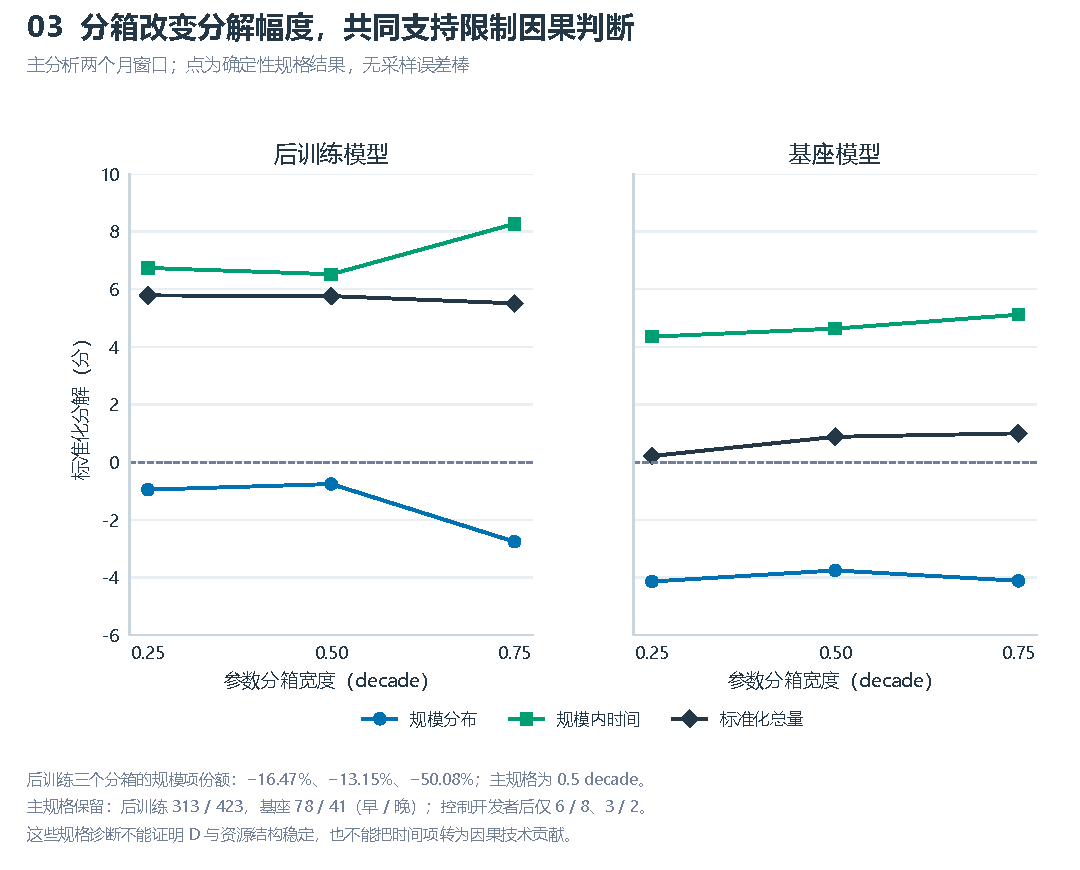
\includegraphics[width=0.84\linewidth]{figures/Q4/03_sensitivity.pdf}
 \caption{参数格宽度变化下的规模分布与同格变化}
 \label{fig:q4-decomp-sensitivity}
\end{figure}

\subsection{算力放缓下的能力前沿}

\subsubsection{预测对象与模型比较}

为描述高分模型群的典型上沿，令 $F_t$ 为同类型模型在截至 $t$ 的最近两个自然月中，式\eqref{eq:q4-score}的第 90 百分位。采用两个月窗口可以降低单个极端记录的影响，同时保留近期变化。观测截点处，后训练组 $F_0=40.445$ 分，基础预训练组为 21.032 分。本文对二者分别预测，并在下一节单独处理“截至目标日的累计最高分”。

设 $z_i=\operatorname{logit}(S_i/100)$，$t_i$ 为距统一基日的月数；对恰为 0 或 100 分的边界值，先将得分比例限制在 $[0.001,0.999]$ 内。分别建立常数基线、两月前沿趋势、均值资源模型，以及以 $\tau=0.9$ 为目标的分位资源模型\cite{koenker2017}。最后一种模型求解
\begin{equation}
 \min_{a,b_N,b_t}\sum_i\rho_{0.9}
 \left[z_i-a-b_N\log_{10}N_i-b_tt_i\right],\qquad
 \rho_\tau(u)=u\{\tau-\mathbf1(u<0)\},
 \label{eq:q4-quantile-fit}
\end{equation}
并采用线性规划得到系数。均值资源模型使用相同解释变量拟合均值关系，两月趋势仅利用历史 $F_t$ 的时间轨迹。四个候选都以未来两个完整自然月的 $F_t$ 为比较目标：每一轮仅用测试窗口开始前的提交版本和当时可见的 C4 资源记录拟合，再计算测试窗口误差\cite{forecasting2021}。

表\ref{tab:q4-backtest}与图\ref{fig:q4-backtests}给出四个滚动窗口的结果。后训练组分位资源模型 RMSE 为 2.199 分，略低于均值资源模型的 2.237；基础组则以常数模型的 7.633 分最低。全部候选的测试 $R^2$ 均为负值，四个窗口还存在重叠，因此该比较用于选择情景模型及观察误差，不据此推定长期预测精度。

\begin{table}[htbp]
 \centering\small
 \caption{最近两月能力前沿的四窗口滚动预测 RMSE（分）}
 \label{tab:q4-backtest}
 \begin{tabular}{lrrrr}
 \toprule
 类型 & 常数 & 两月趋势 & 均值资源 & 分位资源\\
 \midrule
 后训练 & 3.737 & 3.053 & 2.237 & 2.199\\
 基础预训练 & 7.633 & 9.571 & 9.763 & 10.561\\
 \bottomrule
 \end{tabular}
\end{table}

\begin{figure}[htbp]
 \centering
 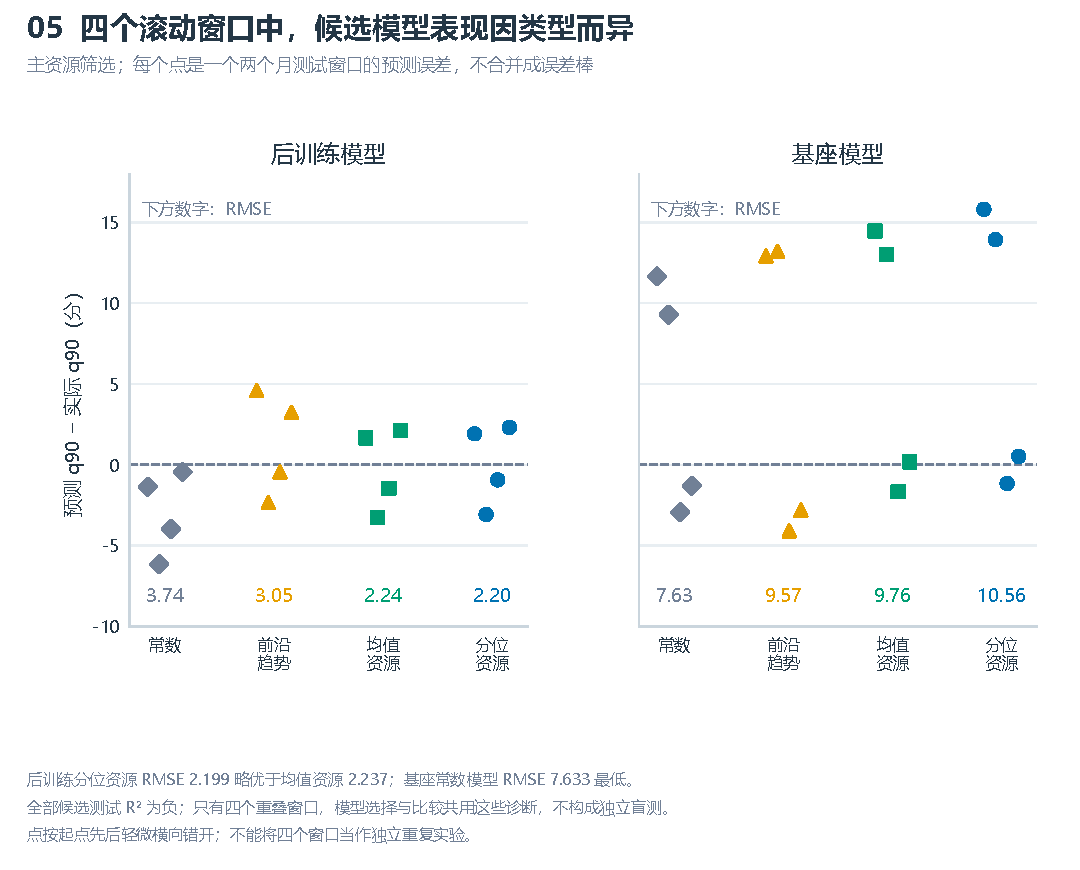
\includegraphics[width=0.85\linewidth]{figures/Q4/05_backtests.pdf}
 \caption{两类模型的最近两月能力前沿滚动预测误差}
 \label{fig:q4-backtests}
\end{figure}

\subsubsection{资源配置情景与前沿预测}

后训练组采用分位资源模型作为主情景。设 $g_C$ 为 C4 的年算力对数增长率，$s$ 为未来增长倍率；取 $s=1,1/2,1/4,0$ 分别表示沿历史速率、增速减半、增速降至四分之一和停止增长。令 $\eta=0.5$ 表示新增资源的一半按十进对数分配给参数量，其余对应训练量；令 $\lambda=0.5$ 为未来时间项的保留系数。以当前两月 $F_0$ 为锚，预测式为
\begin{equation}
 \widehat F(H;s)=100\,\sigma\!\left[
 \operatorname{logit}(F_0/100)
 +b_N\eta s g_C\frac{H}{12}
 +\lambda b_tH\right],\qquad
 \sigma(x)=\frac{1}{1+e^{-x}}.
 \label{eq:q4-frontier-forecast}
\end{equation}
其中 $H$ 为距观测截点的月份。C2 未提供逐模型训练量，故 $\eta$ 是资源分配情景而非由能力数据单独估计的参数。算力增速减半指年对数速率由 0.6903 降至约 0.3452，年倍率由 4.901 降至约 2.214。

后训练组的最后观测日为 2025 年 3 月 13 日。按增速减半，2026 年 3 月 13 日的 12 个月 $F$ 预测为 53.828 分，2027 年 3 月 13 日的 24 个月预测为 66.681 分；其余增长情景列于表\ref{tab:q4-growth}。将 C4 资源核对范围由主口径放宽后，后训练组分位资源模型的四窗 RMSE 为 2.195 分，增速减半时的 12、24 个月预测为 53.222 和 65.591 分，与主口径接近。基础组最后观测日为 2025 年 3 月 9 日，短期比较选择了常数模型，对应的两月第 90 百分位参考值为 21.032 分。图\ref{fig:q4-forecasts}并列显示两类模型的预测。所列日期均从附件观测截点起算。

\begin{table}[htbp]
 \centering\small
 \caption{后训练模型在不同算力增长情景下的两月第 90 百分位预测（分）}
 \label{tab:q4-growth}
 \begin{tabular}{lrrrr}
 \toprule
 预测期限 & 停止增长 & 历史增速的四分之一 & 历史增速减半 & 保持历史增速\\
 \midrule
 12 个月 & 49.157 & 51.496 & 53.828 & 58.432\\
 24 个月 & 57.921 & 62.403 & 66.681 & 74.422\\
 \bottomrule
 \end{tabular}
\end{table}

\begin{figure}[htbp]
 \centering
 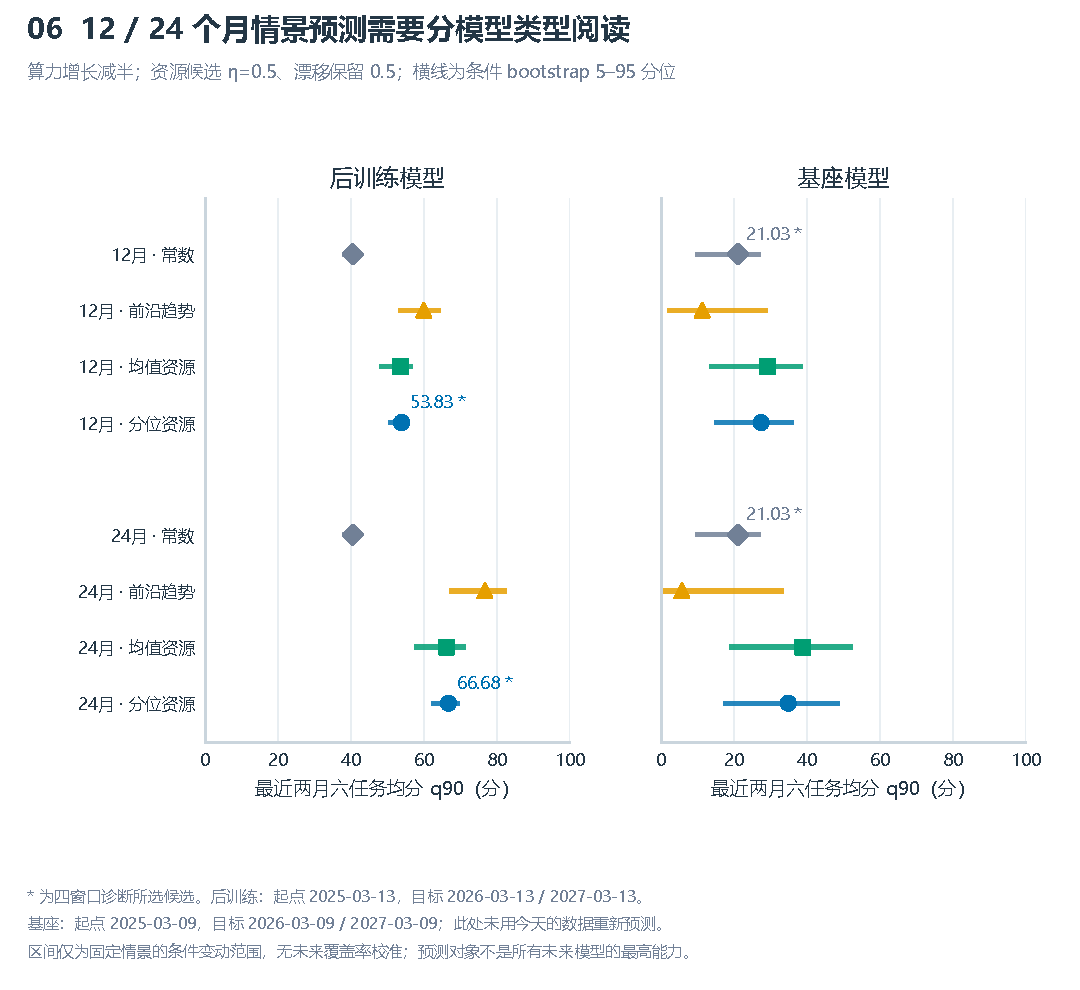
\includegraphics[width=0.86\linewidth]{figures/Q4/06_forecasts.pdf}
 \caption{算力增速减半时两类模型的 12 个月与 24 个月前沿情景}
 \label{fig:q4-forecasts}
\end{figure}

\subsubsection{预测范围与外推程度}

为区分参数扰动和建模情景，先按开发者为单位重复抽取 80 次，在固定增速减半、资源分配及时间保留系数下重新估计，得到后训练组 12 个月的第 5 至第 95 百分位范围 $50.302$--$56.007$ 分，24 个月为 $61.983$--$69.805$ 分。随后改变候选模型、资源筛选、增长速率、$\eta$、$\lambda$、近期窗口及分位水平，取各情景条件范围的并集；最后将四窗口最大绝对误差作为固定偏差压力叠加。表\ref{tab:q4-uncertainty}与图\ref{fig:q4-uncertainty}显示三层范围逐步扩大。它们分别回答“固定参数下怎样波动”“合理情景改变后差多少”“若延续已见偏差会怎样”，尚未用未来观测校准覆盖率。

\begin{table}[htbp]
 \centering\small
 \caption{后训练模型、算力增速减半下的三层条件范围（分）}
 \label{tab:q4-uncertainty}
 \begin{tabular}{lrrr}
 \toprule
 期限 & 固定情景块抽样 & 多情景条件并集 & 叠加固定偏差压力\\
 \midrule
 12 个月 & 50.302--56.007 & 37.755--72.236 & 31.590--78.400\\
 24 个月 & 61.983--69.805 & 37.755--90.640 & 31.590--96.805\\
 \bottomrule
 \end{tabular}
\end{table}

\begin{figure}[htbp]
 \centering
 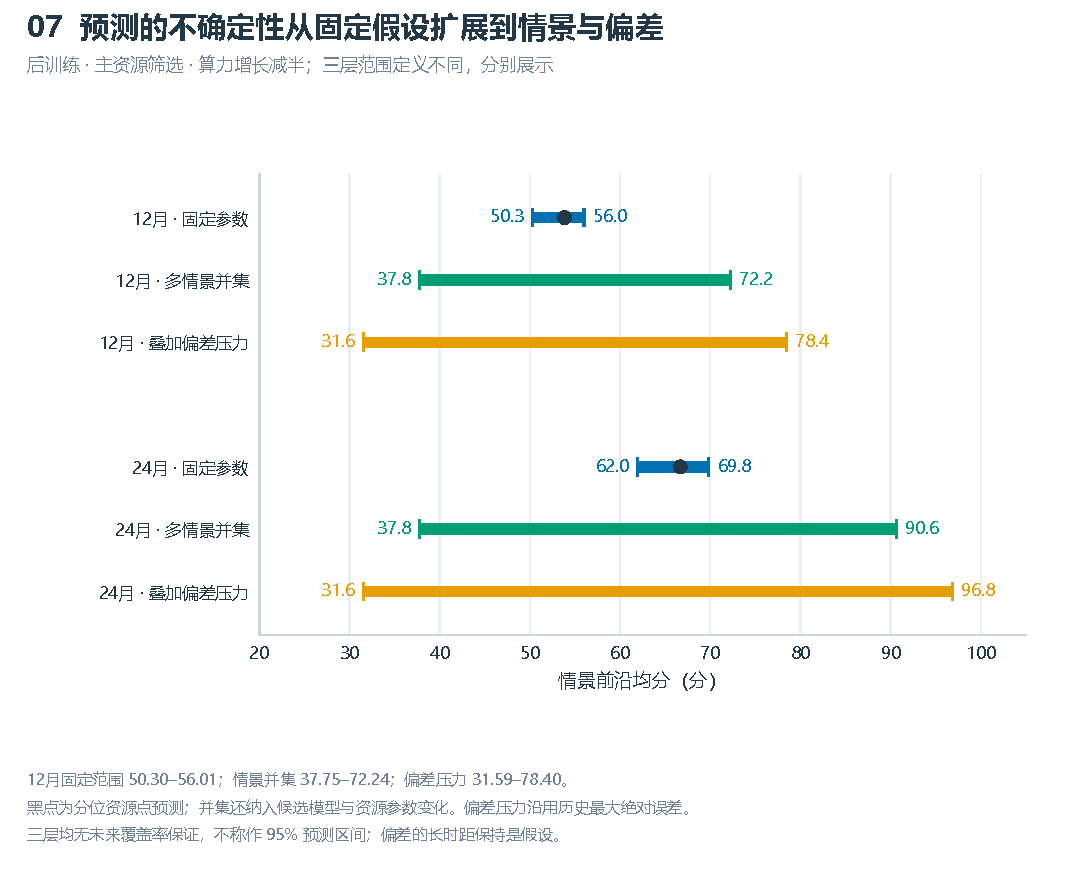
\includegraphics[width=0.85\linewidth]{figures/Q4/07_uncertainty.pdf}
 \caption{固定情景、多情景与偏差压力下的能力前沿范围}
 \label{fig:q4-uncertainty}
\end{figure}

24 个月预测期限约为后训练组已观测时间跨度的 2.64 倍，因此表中长期范围随模型和情景变化显著扩大。近期第 90 百分位描述的是高分模型群，并不直接回答“截至未来目标日的最高分”，下节另建立最高能力边界。

\subsection{截至目标日的最高能力边界}

令 $R_t=\max_{i:d_i\leq t}S_i$ 表示截止日期 $t$ 以前，同一开放筛选和模型类型下所有已提交版本的累计最高分。它至少保持已达到的历史纪录。以纪录保持作为基线，并在式\eqref{eq:q4-frontier-forecast}的第 90 百分位预测之上，加入近期最高分相对第 90 百分位的差额，构造另一种条件上尾情景：
\begin{equation}
 \widehat R^{\rm base}_{t+H}=R_t,\qquad
 \widehat R^{\rm tail}_{t+H}(w)=
 \min\!\left\{100,\max\left[R_t,
 \widehat F(H)+\Delta_{\rm tail}(w)\right]\right\},
 \label{eq:q4-maximum}
\end{equation}
其中 $\Delta_{\rm tail}(w)$ 是最近 $w$ 个月样本最高分与同期第 90 百分位之差，主情景用 $w=2$，并以 1、3 个月比较尾差变化。两项分别表示“不刷新纪录”的经验基线和“近期上尾差额继续存在”的条件方案。

四个重叠的两月回测窗口均未刷新此前累计纪录，故纪录保持基线在这些窗口的 RMSE 为 0；后训练组 1、2、3 月尾差方案的 RMSE 分别为 3.376、2.254、3.683 分。这一短期结果支持将纪录保持作为基线，同时保留上尾情景考察未来可能的纪录更新。算力增速减半时，后训练组当前累计最高分为 51.231，12、24 个月的条件最高边界分别为 60.600 和 73.453 分；将尾差窗口改为 1 或 3 个月，相应范围分别为 60.474--61.203 与 73.327--74.057 分。基础预训练组当前累计最高分 38.441，在其常数前沿情景下两期均保持该值，见表\ref{tab:q4-maximum}和图\ref{fig:q4-maximum}。这些范围反映尾差取法的变化，而非预测误差的概率区间。

\begin{table}[htbp]
 \centering\small
 \caption{算力增速减半时的近期高分群与累计最高能力（分）}
 \label{tab:q4-maximum}
 \begin{tabular}{lrrrrr}
 \toprule
 类型 & 当前纪录 & 12 月 $F$ & 12 月条件最高 & 24 月 $F$ & 24 月条件最高\\
 \midrule
 后训练 & 51.231 & 53.828 & 60.600 & 66.681 & 73.453\\
 基础预训练 & 38.441 & 21.032 & 38.441 & 21.032 & 38.441\\
 \bottomrule
 \end{tabular}
\end{table}

\begin{figure}[htbp]
 \centering
 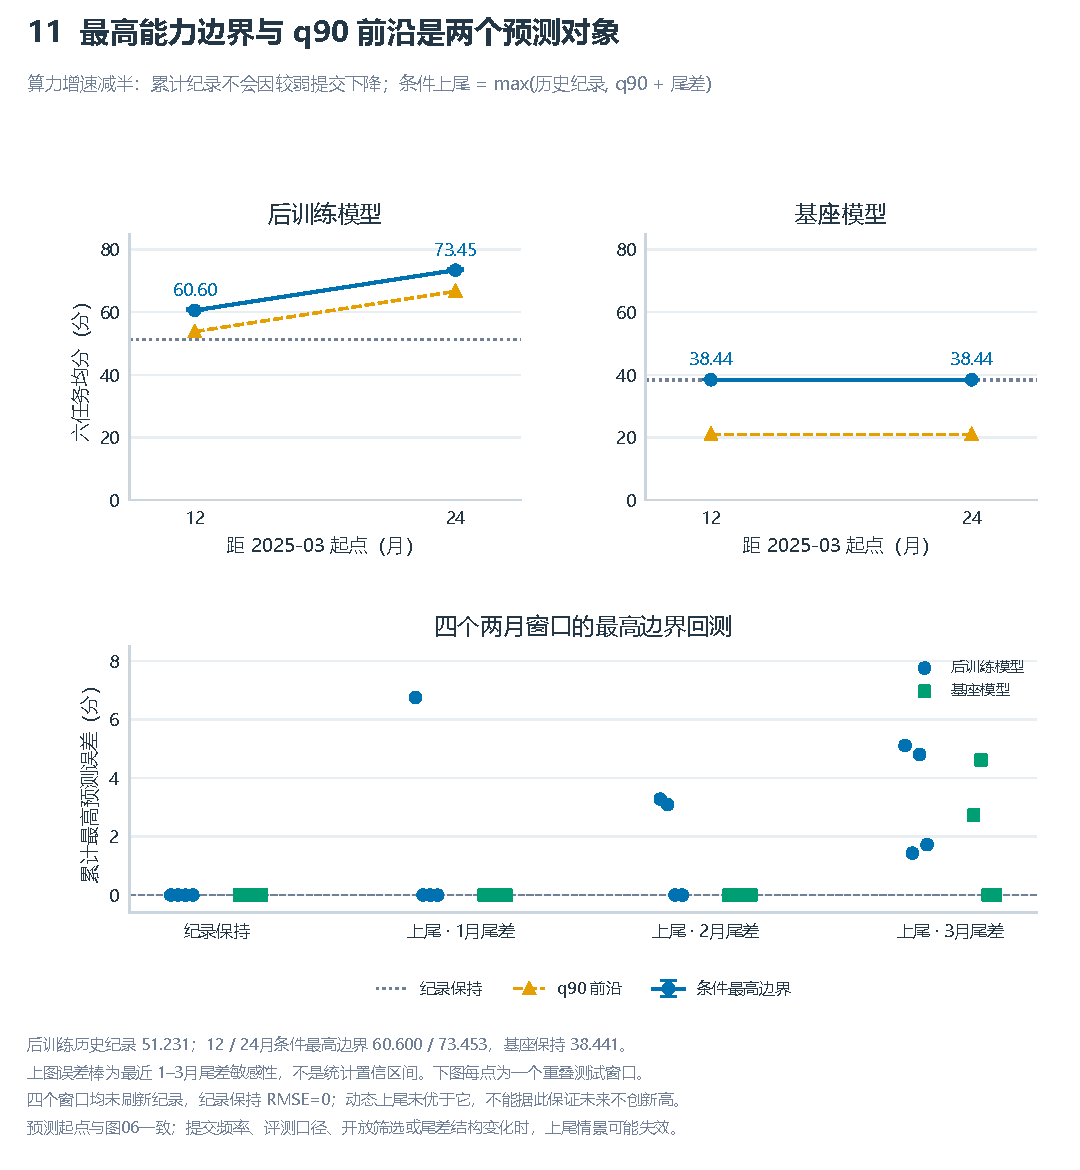
\includegraphics[width=0.85\linewidth]{figures/Q4/11_maximum_boundary.pdf}
 \caption{最近两月高分群、纪录保持基线和条件最高能力边界}
 \label{fig:q4-maximum}
\end{figure}

\subsection{Loss 与能力得分的连接}

\subsubsection{来源内单调映射及检验}

C6 的 Loss 来自不同模型、验证语料和训练阶段。将来源及 Loss 类型分别保留，在每个具有足够成对记录的来源 $s$ 内建立有界的单调关系
\begin{equation}
 \operatorname{logit}\!\left(\frac{S}{100}\right)
 =a_s+b_s\ell_s,\qquad b_s\leq0,
 \label{eq:q4-bridge}
\end{equation}
其中 $\ell_s$ 为该来源记录的 Loss。若估计斜率不满足 Loss 降低、能力提高的方向，模型退回来源内常数关系。对来源内每条记录依次留出、重拟合并预测，同时与常数关系比较。表\ref{tab:q4-bridge-validation}及图\ref{fig:q4-bridge-validation}给出具有 validation 标签的三个主要来源。Qwen2 和 Qwen2.5 的单调关系优于各自常数对照；Pythia 虽具有较高的来源可比性，其小样本关系在留一预测中反而略差。附件的 validation 标签用于区分数据口径，尚不足以建立与第三问 Loss 的直接数值等价。

\begin{table}[htbp]
 \centering\small
 \caption{C6 同来源 Loss--能力映射的逐点留出 RMSE（分）}
 \label{tab:q4-bridge-validation}
 \begin{tabular}{lrrr}
 \toprule
 来源 & 样本数 & 单调关系 & 来源内常数\\
 \midrule
 Pythia validation & 7 & 0.538 & 0.426\\
 Qwen2 validation & 4 & 7.048 & 10.708\\
 Qwen2.5 validation & 6 & 2.655 & 15.074\\
 \bottomrule
 \end{tabular}
\end{table}

\begin{figure}[htbp]
 \centering
 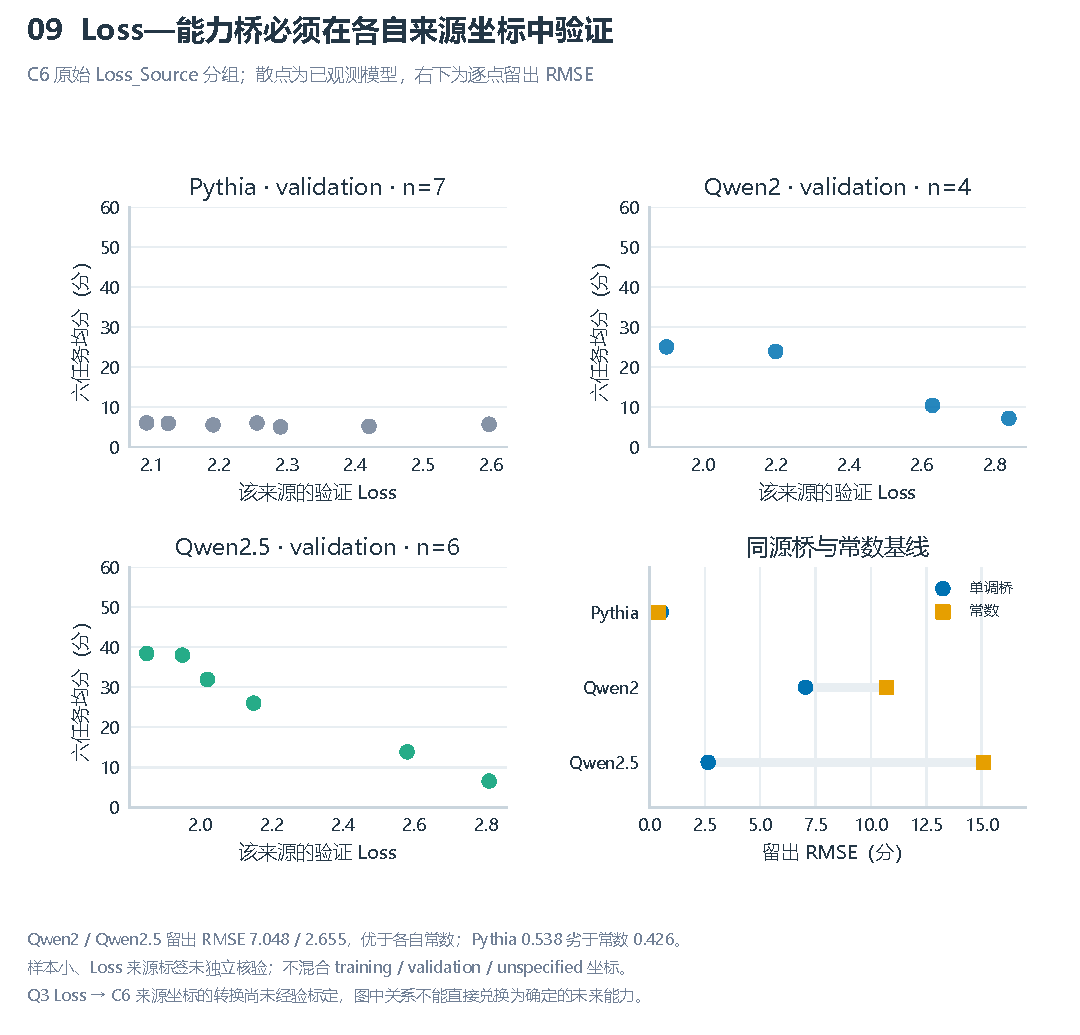
\includegraphics[width=0.85\linewidth]{figures/Q4/09_bridge_validation.pdf}
 \caption{C6 各来源的 Loss--能力关系及逐点留出误差}
 \label{fig:q4-bridge-validation}
\end{figure}

\subsubsection{第三问配置的条件能力换算}

第三问输出的 Loss 与 C6 各来源的 Loss 尚无成对标定。为考察数值换算对这一差异的敏感程度，分别给出正尺度、偏移及上游预测扰动情景
\begin{equation}
 \ell_s=a\{\widehat L_{\rm Q3}+\delta\}+b,
 \quad a\in\{0.9,1,1.1\},\quad
 b\in\{-0.1,0,0.1\},\quad
 \delta\in\{-0.05,0,0.05\}.
 \label{eq:q4-coordinate}
\end{equation}
仅当 $N$ 及变换后的 $\ell_s$ 都位于该来源的观测范围，才代入式\eqref{eq:q4-bridge}。对第三问固定配方、已观测配方联立和独立质量三类配置，分别在五种可拟合的 C6 来源内施加 27 组坐标与上游 Loss 变化。这些区间反映连接假设改变后的结果范围。

以 8192 Token、幂函数质量成本、$10^{22}$ FLOPs 下第三问选择的配方 172 为例，其预测 Loss 为 2.094421。表\ref{tab:q4-bridge-stress}和图\ref{fig:q4-bridge-stress}展示 Qwen2 与 Qwen2.5 两个来源内有观测支持的换算。取 $a=1,b=\delta=0$，预测得分分别为 22.371 与 28.695；改变坐标假设后，前者在 22/27 个可换算情景中为 13.601--27.462，后者在 23/27 个情景中为 15.057--39.197。与相同 $N$ 的规模主干模型相比，模型内得分差在这些可换算情景中保持正值，但其幅度与来源内留出误差处于相近量级，尚需同坐标实验辨别真实改善。

\begin{table}[htbp]
 \centering\small
 \caption{$10^{22}$ FLOPs 下配方 172 的条件得分与坐标变化范围（分）}
 \label{tab:q4-bridge-stress}
 \begin{tabular}{lrrrr}
 \toprule
 C6 来源 & 可换算格 & 名义得分 & 得分范围 & 对规模主干的得分差\\
 \midrule
 Qwen2 validation & 22/27 & 22.371 & 13.601--27.462 & 0.322--3.596\\
 Qwen2.5 validation & 23/27 & 28.695 & 15.057--39.197 & 0.473--5.734\\
 \bottomrule
 \end{tabular}
\end{table}

\begin{figure}[htbp]
 \centering
 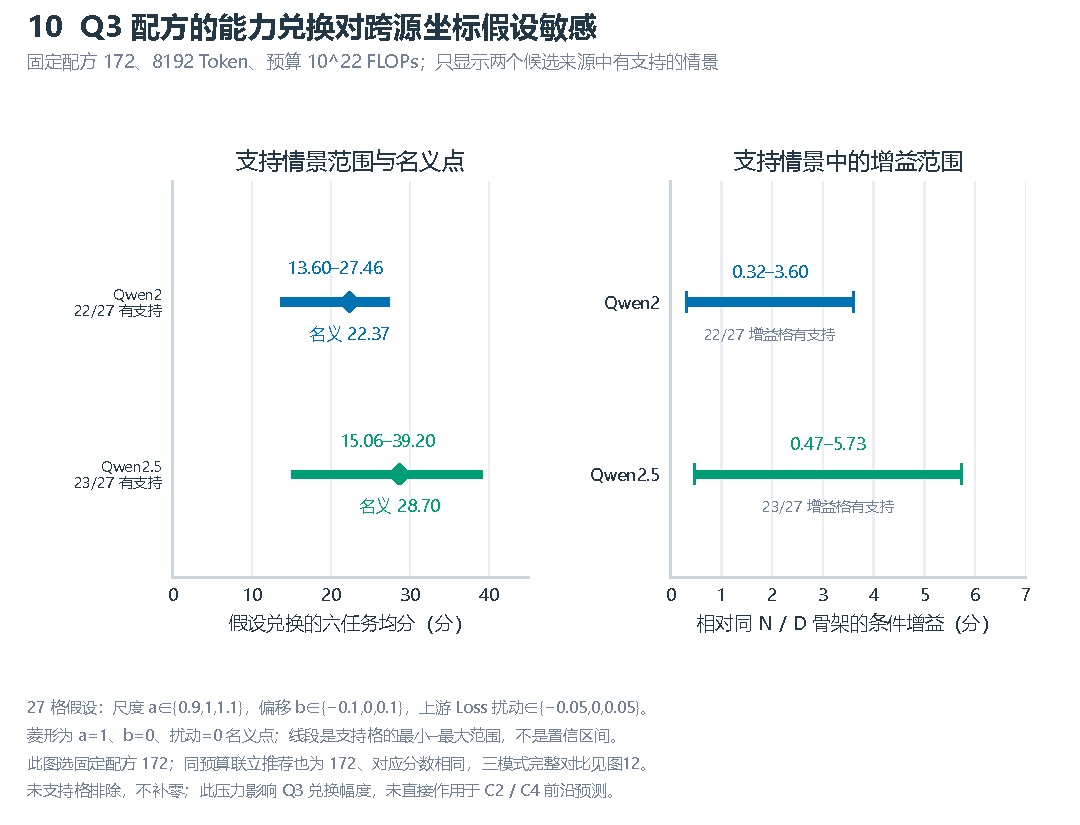
\includegraphics[width=0.85\linewidth]{figures/Q4/10_bridge_stress.pdf}
 \caption{配方 172 在不同 Loss 坐标假设下的能力得分与增量}
 \label{fig:q4-bridge-stress}
\end{figure}

图\ref{fig:q4-policy-bridge}进一步把第三问的三种投入方式放在相同来源坐标情景中比较。$10^{19}$ FLOPs 下固定配方 172 在部分成本设置中不可行；8192 Token、幂成本下联立配方 477 的 $N=0.0873$ 十亿，独立质量方案的 $N=0.1309$ 十亿，均低于 Qwen2 与 Qwen2.5 来源中的最小参数量，故该预算没有相应得分。到 $10^{22}$ 和 $10^{24}$ FLOPs，固定配方与联立配置均选择配方 172，二者在相同情景下得分重合。独立质量方案在 $10^{22}$ FLOPs 下的名义得分为 Qwen2 的 24.489 和 Qwen2.5 的 32.081 分；它改变了质量输入机制，数值差异应与这一前提同时阅读。扩展到全部配方、成本与来源组合时，部分方案相对规模主干的增量在坐标变化中改变符号，方案间排序也会改变。因此，第三问方案的得分比较须与来源和坐标假设一同给出；直接由 C2/C4 拟合的能力前沿式\eqref{eq:q4-frontier-forecast}则不涉及这一换算。

\begin{center}
 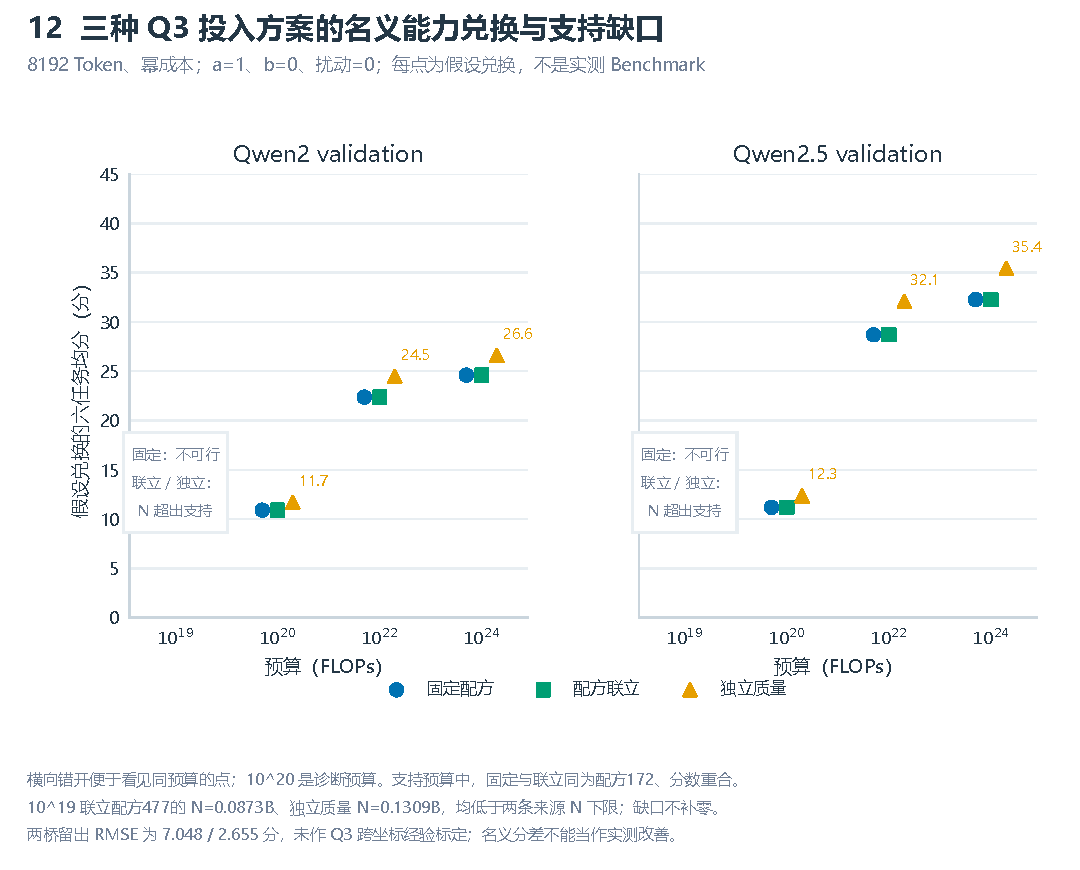
\includegraphics[width=0.80\linewidth]{figures/Q4/12_policy_bridge.pdf}
 \captionof{figure}{三种第三问资源配置在两种 C6 来源中的条件得分}
 \label{fig:q4-policy-bridge}
\end{center}

\subsection{本问输出与结果讨论}

表\ref{tab:q4-output}汇总历史分解、情景预测与第三问方案换算，并注明各结果的使用条件。

\begin{table}[htbp]
 \centering\small
 \caption{问题四的主要结果及跨问题使用方式}
 \label{tab:q4-output}
 \begin{tabular}{p{2.5cm}p{4.2cm}p{5.8cm}}
 \toprule
 结果 & 数值或模型 & 使用方式\\
 \midrule
 历史能力分解 & 后训练组参数分布 $-0.758$ 分，同格变化 6.521 分 & 描述共同支持样本的变化；开放筛选改变时须重新计算\\
 近期高分群 & 增速减半时 12/24 月第 90 百分位 53.828/66.681 分 & 作为后训练模型资源情景下的能力预测\\
 累计最高能力 & 纪录保持 51.231 分；条件上尾 60.600/73.453 分 & 分别提供已达到的基线和未来刷新纪录的情景\\
 Loss--能力联系 & C6 来源内单调映射及逐点留出误差 & 先核对来源与参数、Loss 范围，再比较第三问配置\\
 配方换算 & 配方 172 的两来源名义得分 22.371/28.695 分 & 仅在明示 Loss 坐标假设下讨论方案得分与排序\\
 \bottomrule
 \end{tabular}
\end{table}

综上，参数格标准化分解刻画了历史能力增长中的规模分布与同格变化；资源情景模型分别给出近期高分群和累计最高能力的未来参考值。来源内 Loss--能力关系进一步连接了第三问的训练配置，配方得分随 Loss 坐标假设而变化。上述结果为分析开源模型能力演进及不同算力路径下的训练方案提供了定量依据。
